\tikzset{every picture/.style={line width=0.75pt}} %set default line width to 0.75pt        

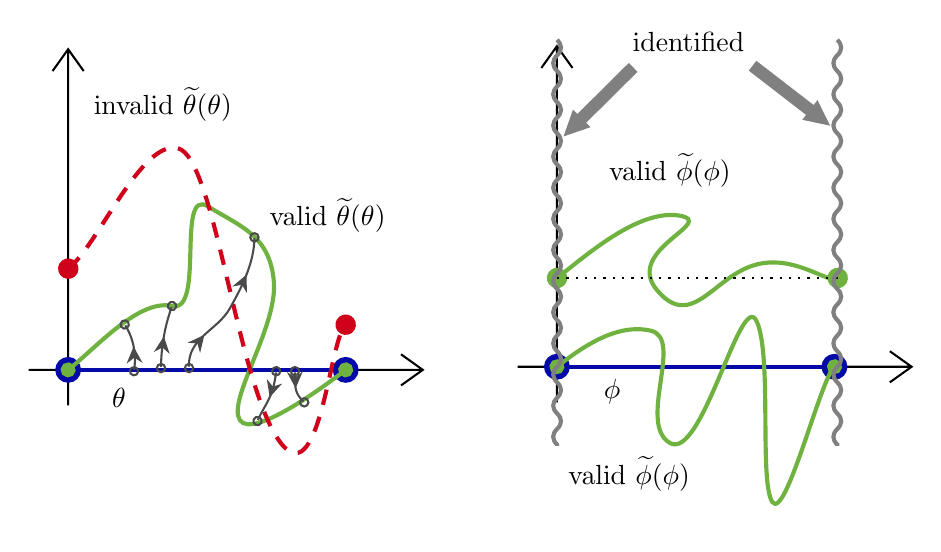
\begin{tikzpicture}[x=0.75pt,y=0.75pt,yscale=-1.5,xscale=1.5]
%uncomment if require: \path (0,310); %set diagram left start at 0, and has height of 310

%Shape: Axis 2D [id:dp25002381159098763] 
\draw  (15,115.58) -- (141.59,115.58)(27.66,12.6) -- (27.66,127.02) (134.59,110.58) -- (141.59,115.58) -- (134.59,120.58) (22.66,19.6) -- (27.66,12.6) -- (32.66,19.6)  ;
%Straight Lines [id:da012448710548571551] 
\draw [color={rgb, 255:red, 3; green, 10; blue, 167 }  ,draw opacity=1 ][line width=1.5]    (27.66,115.58) -- (116.81,115.58) ;
\draw [shift={(116.81,115.58)}, rotate = 0] [color={rgb, 255:red, 3; green, 10; blue, 167 }  ,draw opacity=1 ][fill={rgb, 255:red, 3; green, 10; blue, 167 }  ,fill opacity=1 ][line width=1.5]      (0, 0) circle [x radius= 3.48, y radius= 3.48]   ;
\draw [shift={(27.66,115.58)}, rotate = 0] [color={rgb, 255:red, 3; green, 10; blue, 167 }  ,draw opacity=1 ][fill={rgb, 255:red, 3; green, 10; blue, 167 }  ,fill opacity=1 ][line width=1.5]      (0, 0) circle [x radius= 3.48, y radius= 3.48]   ;
%Curve Lines [id:da22036725062847506] 
\draw [color={rgb, 255:red, 112; green, 178; blue, 63 }  ,draw opacity=1 ][line width=1.5]    (27.66,115.58) .. controls (36.47,108.71) and (50.34,92.65) .. (61.04,95.07) .. controls (71.74,97.5) and (62.19,56.64) .. (72.58,63.08) .. controls (82.97,69.52) and (92.41,72.35) .. (93.73,87.07) .. controls (95.05,101.79) and (78.57,125.26) .. (82.84,131.73) .. controls (87.1,138.21) and (112.47,118.96) .. (116.81,115.58) ;
\draw [shift={(116.81,115.58)}, rotate = 322.05] [color={rgb, 255:red, 112; green, 178; blue, 63 }  ,draw opacity=1 ][fill={rgb, 255:red, 112; green, 178; blue, 63 }  ,fill opacity=1 ][line width=1.5]      (0, 0) circle [x radius= 1.74, y radius= 1.74]   ;
\draw [shift={(27.66,115.58)}, rotate = 322.05] [color={rgb, 255:red, 112; green, 178; blue, 63 }  ,draw opacity=1 ][fill={rgb, 255:red, 112; green, 178; blue, 63 }  ,fill opacity=1 ][line width=1.5]      (0, 0) circle [x radius= 1.74, y radius= 1.74]   ;
%Curve Lines [id:da5448767767433973] 
\draw [color={rgb, 255:red, 208; green, 2; blue, 27 }  ,draw opacity=1 ][line width=1.5]  [dash pattern={on 5.63pt off 4.5pt}]  (27.71,83.07) .. controls (37.31,75.59) and (51.22,41.38) .. (62.97,44.42) .. controls (74.71,47.45) and (81.52,117.49) .. (95.01,137.73) .. controls (108.51,157.97) and (111.6,105.13) .. (116.81,101.07) ;
\draw [shift={(116.81,101.07)}, rotate = 322.05] [color={rgb, 255:red, 208; green, 2; blue, 27 }  ,draw opacity=1 ][fill={rgb, 255:red, 208; green, 2; blue, 27 }  ,fill opacity=1 ][line width=1.5]      (0, 0) circle [x radius= 2.61, y radius= 2.61]   ;
\draw [shift={(27.71,83.07)}, rotate = 322.05] [color={rgb, 255:red, 208; green, 2; blue, 27 }  ,draw opacity=1 ][fill={rgb, 255:red, 208; green, 2; blue, 27 }  ,fill opacity=1 ][line width=1.5]      (0, 0) circle [x radius= 2.61, y radius= 2.61]   ;
%Shape: Axis 2D [id:dp20850113919583269] 
\draw  (172,114.58) -- (298.59,114.58)(184.66,11.6) -- (184.66,126.02) (291.59,109.58) -- (298.59,114.58) -- (291.59,119.58) (179.66,18.6) -- (184.66,11.6) -- (189.66,18.6)  ;
%Straight Lines [id:da009943316285294879] 
\draw [color={rgb, 255:red, 3; green, 10; blue, 167 }  ,draw opacity=1 ][line width=1.5]    (184.66,114.58) -- (273.81,114.58) ;
\draw [shift={(273.81,114.58)}, rotate = 0] [color={rgb, 255:red, 3; green, 10; blue, 167 }  ,draw opacity=1 ][fill={rgb, 255:red, 3; green, 10; blue, 167 }  ,fill opacity=1 ][line width=1.5]      (0, 0) circle [x radius= 3.48, y radius= 3.48]   ;
\draw [shift={(184.66,114.58)}, rotate = 0] [color={rgb, 255:red, 3; green, 10; blue, 167 }  ,draw opacity=1 ][fill={rgb, 255:red, 3; green, 10; blue, 167 }  ,fill opacity=1 ][line width=1.5]      (0, 0) circle [x radius= 3.48, y radius= 3.48]   ;
%Curve Lines [id:da9273036543894462] 
\draw [color={rgb, 255:red, 112; green, 178; blue, 63 }  ,draw opacity=1 ][line width=1.5]    (184.66,114.58) .. controls (193.47,107.71) and (204.13,100.57) .. (214.83,103) .. controls (225.54,105.43) and (210.44,132.56) .. (220.83,139) .. controls (231.23,145.44) and (243.83,89) .. (248.83,100) .. controls (253.83,111) and (249.57,151.53) .. (253.83,158) .. controls (258.1,164.47) and (269.47,117.96) .. (273.81,114.58) ;
\draw [shift={(273.81,114.58)}, rotate = 322.05] [color={rgb, 255:red, 112; green, 178; blue, 63 }  ,draw opacity=1 ][fill={rgb, 255:red, 112; green, 178; blue, 63 }  ,fill opacity=1 ][line width=1.5]      (0, 0) circle [x radius= 1.74, y radius= 1.74]   ;
\draw [shift={(184.66,114.58)}, rotate = 322.05] [color={rgb, 255:red, 112; green, 178; blue, 63 }  ,draw opacity=1 ][fill={rgb, 255:red, 112; green, 178; blue, 63 }  ,fill opacity=1 ][line width=1.5]      (0, 0) circle [x radius= 1.74, y radius= 1.74]   ;
%Curve Lines [id:da4879760234687782] 
\draw [color={rgb, 255:red, 112; green, 178; blue, 63 }  ,draw opacity=1 ][line width=1.5]    (184.71,86.07) .. controls (194.31,78.59) and (210.83,64) .. (223.83,66) .. controls (236.83,68) and (205.83,77) .. (216.83,90) .. controls (227.83,103) and (234.83,86) .. (247.83,82) .. controls (260.83,78) and (271.94,88.33) .. (274.83,86.07) ;
\draw [shift={(274.83,86.07)}, rotate = 322.05] [color={rgb, 255:red, 112; green, 178; blue, 63 }  ,draw opacity=1 ][fill={rgb, 255:red, 112; green, 178; blue, 63 }  ,fill opacity=1 ][line width=1.5]      (0, 0) circle [x radius= 2.61, y radius= 2.61]   ;
\draw [shift={(184.71,86.07)}, rotate = 322.05] [color={rgb, 255:red, 112; green, 178; blue, 63 }  ,draw opacity=1 ][fill={rgb, 255:red, 112; green, 178; blue, 63 }  ,fill opacity=1 ][line width=1.5]      (0, 0) circle [x radius= 2.61, y radius= 2.61]   ;
%Straight Lines [id:da4922067466008355] 
\draw  [dash pattern={on 0.84pt off 2.51pt}]  (184.71,86.07) -- (274.83,86.07) ;
%Straight Lines [id:da19681082381448634] 
\draw [color={rgb, 255:red, 128; green, 128; blue, 128 }  ,draw opacity=1 ][line width=1.5]    (184.71,9.57) .. controls (186.38,11.24) and (186.38,12.9) .. (184.71,14.57) .. controls (183.04,16.24) and (183.04,17.9) .. (184.71,19.57) .. controls (186.38,21.24) and (186.38,22.9) .. (184.71,24.57) .. controls (183.04,26.24) and (183.04,27.9) .. (184.71,29.57) .. controls (186.38,31.24) and (186.38,32.9) .. (184.71,34.57) .. controls (183.04,36.24) and (183.04,37.9) .. (184.71,39.57) .. controls (186.38,41.24) and (186.38,42.9) .. (184.71,44.57) .. controls (183.04,46.24) and (183.04,47.9) .. (184.71,49.57) .. controls (186.38,51.24) and (186.38,52.9) .. (184.71,54.57) .. controls (183.04,56.24) and (183.04,57.9) .. (184.71,59.57) .. controls (186.38,61.24) and (186.38,62.9) .. (184.71,64.57) .. controls (183.04,66.24) and (183.04,67.9) .. (184.71,69.57) .. controls (186.38,71.24) and (186.38,72.9) .. (184.71,74.57) .. controls (183.04,76.24) and (183.04,77.9) .. (184.71,79.57) .. controls (186.38,81.24) and (186.38,82.9) .. (184.71,84.57) .. controls (183.04,86.24) and (183.04,87.9) .. (184.71,89.57) .. controls (186.38,91.24) and (186.38,92.9) .. (184.71,94.57) .. controls (183.04,96.24) and (183.04,97.9) .. (184.71,99.57) .. controls (186.38,101.24) and (186.38,102.9) .. (184.71,104.57) .. controls (183.04,106.24) and (183.04,107.9) .. (184.71,109.57) .. controls (186.38,111.24) and (186.38,112.9) .. (184.71,114.57) .. controls (183.04,116.24) and (183.04,117.9) .. (184.71,119.57) .. controls (186.38,121.24) and (186.38,122.9) .. (184.71,124.57) .. controls (183.04,126.24) and (183.04,127.9) .. (184.71,129.57) .. controls (186.38,131.24) and (186.38,132.9) .. (184.71,134.57) .. controls (183.04,136.24) and (183.04,137.9) .. (184.71,139.57) -- (184.71,140) -- (184.71,140) ;
%Straight Lines [id:da016350095710515156] 
\draw [color={rgb, 255:red, 128; green, 128; blue, 128 }  ,draw opacity=1 ][line width=1.5]    (274.71,9.57) .. controls (276.38,11.24) and (276.38,12.9) .. (274.71,14.57) .. controls (273.04,16.24) and (273.04,17.9) .. (274.71,19.57) .. controls (276.38,21.24) and (276.38,22.9) .. (274.71,24.57) .. controls (273.04,26.24) and (273.04,27.9) .. (274.71,29.57) .. controls (276.38,31.24) and (276.38,32.9) .. (274.71,34.57) .. controls (273.04,36.24) and (273.04,37.9) .. (274.71,39.57) .. controls (276.38,41.24) and (276.38,42.9) .. (274.71,44.57) .. controls (273.04,46.24) and (273.04,47.9) .. (274.71,49.57) .. controls (276.38,51.24) and (276.38,52.9) .. (274.71,54.57) .. controls (273.04,56.24) and (273.04,57.9) .. (274.71,59.57) .. controls (276.38,61.24) and (276.38,62.9) .. (274.71,64.57) .. controls (273.04,66.24) and (273.04,67.9) .. (274.71,69.57) .. controls (276.38,71.24) and (276.38,72.9) .. (274.71,74.57) .. controls (273.04,76.24) and (273.04,77.9) .. (274.71,79.57) .. controls (276.38,81.24) and (276.38,82.9) .. (274.71,84.57) .. controls (273.04,86.24) and (273.04,87.9) .. (274.71,89.57) .. controls (276.38,91.24) and (276.38,92.9) .. (274.71,94.57) .. controls (273.04,96.24) and (273.04,97.9) .. (274.71,99.57) .. controls (276.38,101.24) and (276.38,102.9) .. (274.71,104.57) .. controls (273.04,106.24) and (273.04,107.9) .. (274.71,109.57) .. controls (276.38,111.24) and (276.38,112.9) .. (274.71,114.57) .. controls (273.04,116.24) and (273.04,117.9) .. (274.71,119.57) .. controls (276.38,121.24) and (276.38,122.9) .. (274.71,124.57) .. controls (273.04,126.24) and (273.04,127.9) .. (274.71,129.57) .. controls (276.38,131.24) and (276.38,132.9) .. (274.71,134.57) .. controls (273.04,136.24) and (273.04,137.9) .. (274.71,139.57) -- (274.71,140) -- (274.71,140) ;
%Right Arrow [id:dp761231037087466] 
\draw  [draw opacity=0][fill={rgb, 255:red, 128; green, 128; blue, 128 }  ,fill opacity=1 ] (248.72,16.31) -- (267.13,30.52) -- (268.34,28.94) -- (272.43,37.14) -- (263.47,35.25) -- (264.69,33.68) -- (246.29,19.47) -- cycle ;
%Right Arrow [id:dp13272832472280505] 
\draw  [draw opacity=0][fill={rgb, 255:red, 128; green, 128; blue, 128 }  ,fill opacity=1 ] (210.55,19.84) -- (194.04,36.21) -- (195.45,37.63) -- (186.79,40.6) -- (189.83,31.97) -- (191.24,33.38) -- (207.74,17.01) -- cycle ;
%Curve Lines [id:da07870378678844014] 
\draw [color={rgb, 255:red, 74; green, 74; blue, 74 }  ,draw opacity=1 ]   (48.89,115.58) .. controls (49.73,109) and (47.91,104.23) .. (46.01,101.27) ;
\draw [shift={(45.83,101)}, rotate = 236.31] [color={rgb, 255:red, 74; green, 74; blue, 74 }  ,draw opacity=1 ][line width=0.75]      (0, 0) circle [x radius= 1.34, y radius= 1.34]   ;
\draw [shift={(48.7,108.1)}, rotate = 446.84] [fill={rgb, 255:red, 74; green, 74; blue, 74 }  ,fill opacity=1 ][line width=0.08]  [draw opacity=0] (5.36,-2.57) -- (0,0) -- (5.36,2.57) -- (3.56,0) -- cycle    ;
\draw [shift={(48.83,116)}, rotate = 278.13] [color={rgb, 255:red, 74; green, 74; blue, 74 }  ,draw opacity=1 ][line width=0.75]      (0, 0) circle [x radius= 1.34, y radius= 1.34]   ;
%Curve Lines [id:da7786738388766477] 
\draw [color={rgb, 255:red, 74; green, 74; blue, 74 }  ,draw opacity=1 ]   (57.5,114.64) .. controls (57.54,108.81) and (58.52,102.07) .. (60.93,95.38) ;
\draw [shift={(61.04,95.07)}, rotate = 290.15] [color={rgb, 255:red, 74; green, 74; blue, 74 }  ,draw opacity=1 ][line width=0.75]      (0, 0) circle [x radius= 1.34, y radius= 1.34]   ;
\draw [shift={(58.41,104.84)}, rotate = 457.22] [fill={rgb, 255:red, 74; green, 74; blue, 74 }  ,fill opacity=1 ][line width=0.08]  [draw opacity=0] (5.36,-2.57) -- (0,0) -- (5.36,2.57) -- (3.56,0) -- cycle    ;
\draw [shift={(57.5,115)}, rotate = 270] [color={rgb, 255:red, 74; green, 74; blue, 74 }  ,draw opacity=1 ][line width=0.75]      (0, 0) circle [x radius= 1.34, y radius= 1.34]   ;
%Curve Lines [id:da4539251046582702] 
\draw [color={rgb, 255:red, 74; green, 74; blue, 74 }  ,draw opacity=1 ]   (66.47,114.57) .. controls (66.06,105.35) and (75.56,102.9) .. (79.5,96) .. controls (83.46,89.07) and (87.42,81.16) .. (87.5,73.24) ;
\draw [shift={(87.5,73)}, rotate = 270] [color={rgb, 255:red, 74; green, 74; blue, 74 }  ,draw opacity=1 ][line width=0.75]      (0, 0) circle [x radius= 1.34, y radius= 1.34]   ;
\draw [shift={(71.44,104.33)}, rotate = 489.22] [fill={rgb, 255:red, 74; green, 74; blue, 74 }  ,fill opacity=1 ][line width=0.08]  [draw opacity=0] (5.36,-2.57) -- (0,0) -- (5.36,2.57) -- (3.56,0) -- cycle    ;
\draw [shift={(84.95,84.99)}, rotate = 474.23] [fill={rgb, 255:red, 74; green, 74; blue, 74 }  ,fill opacity=1 ][line width=0.08]  [draw opacity=0] (5.36,-2.57) -- (0,0) -- (5.36,2.57) -- (3.56,0) -- cycle    ;
\draw [shift={(66.5,115)}, rotate = 265.63] [color={rgb, 255:red, 74; green, 74; blue, 74 }  ,draw opacity=1 ][line width=0.75]      (0, 0) circle [x radius= 1.34, y radius= 1.34]   ;
%Curve Lines [id:da11305718845382184] 
\draw [color={rgb, 255:red, 74; green, 74; blue, 74 }  ,draw opacity=1 ]   (94.45,116.4) .. controls (93.43,124.89) and (90.59,126.99) .. (88.62,131.71) ;
\draw [shift={(88.5,132)}, rotate = 111.8] [color={rgb, 255:red, 74; green, 74; blue, 74 }  ,draw opacity=1 ][line width=0.75]      (0, 0) circle [x radius= 1.34, y radius= 1.34]   ;
\draw [shift={(92.4,124.38)}, rotate = 286.65999999999997] [fill={rgb, 255:red, 74; green, 74; blue, 74 }  ,fill opacity=1 ][line width=0.08]  [draw opacity=0] (5.36,-2.57) -- (0,0) -- (5.36,2.57) -- (3.56,0) -- cycle    ;
\draw [shift={(94.5,116)}, rotate = 96.34] [color={rgb, 255:red, 74; green, 74; blue, 74 }  ,draw opacity=1 ][line width=0.75]      (0, 0) circle [x radius= 1.34, y radius= 1.34]   ;
%Curve Lines [id:da9507709065370622] 
\draw [color={rgb, 255:red, 74; green, 74; blue, 74 }  ,draw opacity=1 ]   (100.5,116.35) .. controls (100.5,121.9) and (100.56,123.01) .. (103.28,125.78) ;
\draw [shift={(103.5,126)}, rotate = 45] [color={rgb, 255:red, 74; green, 74; blue, 74 }  ,draw opacity=1 ][line width=0.75]      (0, 0) circle [x radius= 1.34, y radius= 1.34]   ;
\draw [shift={(100.73,121.49)}, rotate = 267.40999999999997] [fill={rgb, 255:red, 74; green, 74; blue, 74 }  ,fill opacity=1 ][line width=0.08]  [draw opacity=0] (5.36,-2.57) -- (0,0) -- (5.36,2.57) -- (3.56,0) -- cycle    ;
\draw [shift={(100.5,116)}, rotate = 90] [color={rgb, 255:red, 74; green, 74; blue, 74 }  ,draw opacity=1 ][line width=0.75]      (0, 0) circle [x radius= 1.34, y radius= 1.34]   ;

% Text Node
\draw (40.76,120.51) node [anchor=north west][inner sep=0.75pt]    {$\theta$};
% Text Node
\draw (34.89,23.86) node [anchor=north west][inner sep=0.75pt]   [align=left] {invalid $\displaystyle \widetilde{\theta }( \theta )$};
% Text Node
\draw (91.37,59.52) node [anchor=north west][inner sep=0.75pt]   [align=left] {valid $\displaystyle \widetilde{\theta }( \theta)$};
% Text Node
\draw (198.76,117.51) node [anchor=north west][inner sep=0.75pt]    {$\phi$};
% Text Node
\draw (200.45,45.03) node [anchor=north west][inner sep=0.75pt]   [align=left] {valid $\displaystyle \widetilde{\phi }( \phi)$};
% Text Node
\draw (187.37,142.52) node [anchor=north west][inner sep=0.75pt]   [align=left] {valid $\displaystyle \widetilde{\phi }( \phi)$};
% Text Node
\draw (208,6) node [anchor=north west][inner sep=0.75pt]   [align=left] {identified};


\end{tikzpicture}